\section{병렬화 운영체제 역사}
%20년의 프로세서들은 단일프로세서(uniprocessor) 디자인을 가졌고, 병렬처리와 락은 필요가 없었다. 
%Goal of an OS interface
%Make application developer's job easy
%Allow sharing
%File system, buffer cache, load balancing, etc.
%But, perfectly scalable Efficient implementation

%Three types of parallelism in operating systems
%1. User parallelism
%Users working concurrently with computer
%2. I/O concurrency
%Overlap computation with I/O to keep a processor busy
%3. Multiprocessors parallelism
%Exploit several processors to speedup tasks
%The first two may involve only 1 processor

%This talk: 4 phases in OS parallelism
%Time sharing
%Client/server
%SMPs
%Multicore 60s/70s
%80s/90s
%90s/2000s
%2005s-now Introduction of many ideas for parallelism
%I/O concurrency inside servers
%Multiprocessor kernels and servers
%All software parallel

%POSIX is just the wrong interface
%Shared data fundamentally limits scalability
%Kernels are too big/complex to fix
%Designs cannot keep up with core count

본 장에서는 현시점에서 운영체제 병렬화가 필요한 이유와 함께 운영체제의 병렬화의 역사에 관해서 설명한다.
그동안 운영체제의 병렬화는 시분활 시스템, 클라이언트(client) 서버(server) 구조, 그리고 SMPs(Shared Memory
Processor) 그리고 최근 프로세서에 코어가 많아 지는 멀티코어로 총 4단계에 거처 발전해 왔다~\cite{Kaashoek2015PCO}.

첫 번째 단계에서는 시분활 시스템에서 사용되는 병렬화이다. 
60년대 부터 70년대에서의 운영체제 병렬성은 시분할(time sharing) 시스템을 가졌다.
즉 컴퓨터 한대에 여러 사용자가 동시에 사용되었고, 대부분이 1개의 프로세서로 이루어졌다.
이 시점에서 병렬 처리 연구는 I/O 병렬화 프로그램에 대한 연구가 진행되었다~\cite{Bloch1959EDS}[CTSS 1962]. 
최대한 프로세서를 이용률(utilization)를 높여서 I/O를 처리하기 위해 즉 커널은
 병렬로 I/O를 처리하기 위해 다른 프로그램 커널로 문맥교환되어 실행되도록 만들었다.
 
%Example: the THE operating system [EWD123 1965, SOSP 1967]
%~\cite{Dijkstra1965CSP}
%Technische Hogeschool Eindhoven (THE)
%OS organized as many “sequential” processes
%I A driver is a sequential process
%The THE solution: semaphores

초기 컴퓨터 중 일부 프로세서들은 시분활 시스템과 멀티프로세서의 병렬화를 고려하여
 만들었다(예를 들어, 버로우스(Burroughs)의 B5000~\cite{Mayer1982ABB}).
따라서, 병렬화에 대해서 많은 관심과 노력이 이루어졌다.
그 결과 병렬화 관련 초기 많은 이론인 암달의 법칙~\cite{Amdahl1967VSP}, 멀틱스(Multics)에서의 트래픽 컨트롤
~\cite{Saltzer1966TCM}, 데드락 발견(deadlock detection) 그리고 락 오더링(locking ordering)등
많은 이론들이 생겨나게 되었다. 
70년대 하나의 프로세서 위에서 병렬화를 제공하기 위해 많은 연구 및 개발이 이루어졌고, 실제 
단일 프로세스에 여러 유저에게 시분활 기능으로
 병렬화를 제공하는 Unix 커널~\cite{Ritchie1973UTS}이 개발되었다.

두번째 단계에서는 80년대와 90년대에는 컴퓨터의 가격이 개인이 구매가 가능할 정도 내려갔으며,
 로컬 네트워크로 여러 유저가 
협업하면서 작업할 수 있는 환경이 되어 클라인트 서버 환경을 위한 병렬화가 이루어졌다.
문제는 여러 유저가 수행할 서비스(services)에 대한 병렬화가 필요하게 되었고, 
따라서 논커널 프로그래머들도 커널의 기능이 필요하여, 서버의 커널이 인터페이스(interface)를
 추가하여 유저들에게 병렬화 서비스를 제공하였다. 
 
그 결과 많은 운영체제 병렬화 기술들이 이 시점에 연구 개발되었다. 
예를 들어 스레드(Thread), 락(Locks) 그리고 컨디션 변수(Condition variables)등 이 시점에 많은 연구가 
이루어졌다.
이벤트(events)와 스레드(threads)에 대한 논쟁~\cite{Ous96}~\cite{vonBehren2003WEB}
그리고 Accent~\cite{Rashid1981ACO},
Mach~\cite{Accetta86mach} , V~\cite{Cheriton1983DVK} 등 새로운 운영체제들이 제안되었다. 
이러한 연구들은 마이크로커널(microkernel)에 영감을 주었고, 결국 최근 많은 운영체제가 사용하고 있는 
Pthreads[POSIX.1c, Threads extensions (IEEE Std 1003.1c-1995)]에 대해 영향을 주었다. 
새로운 운영체제 뿐만 아니라 새로운 언어들(예를들어 Mesa~\cite{Lampson1979EPM})도
 연구되었고, 결국 가비지 컬렉션등에 대한 연구가 같이 진행되어, 그 결과 것들이 최근 자바(JAVA)와 고(Go) 언어등에
 영감을 주었다.
결론으로 커널의 인터페이스를 서버 개발자에게 노출하여 서버를 병렬로 이용 할 수 있게 만들었다.


\begin{figure}[h]
    \centering
    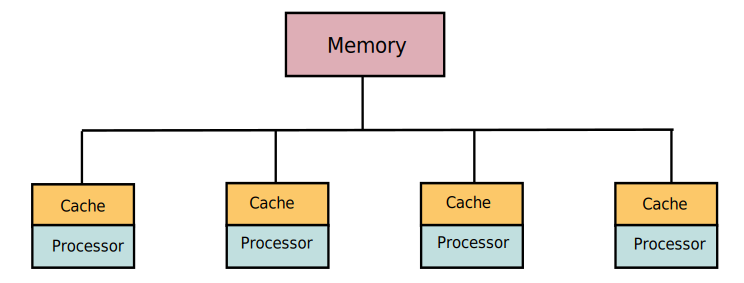
\includegraphics[width=0.8\textwidth]{fig/shared_memory}
    \caption{90년대 공유 메모리 시스템}
  \label{shared_memory}
\end{figure}




다음 단계에서는 90년대 각각의 프로세서가 메모리를 공유하는 개념의 컴퓨터인 SMP(Shared-memory Multi
Pocessors)가 낮은 가격으로 보급이 되어서, 커널 또는 서버 개발자는 이 떄부터 심각하게 운영체제 병렬화에 대해서 고려하게 되었다.
예를 들어, 운영체제 커널은 BKL(Big Kernel Lock) 등을 지원하며 병렬화 기능을 제공하기 시작하였다.
이 시점 많은 회사(BBN Butterfly, Sequent, SGI, Sun, Thinking Machines 등)가 운영체제 병렬화에 대해서 
연구하기 시작했다.
그 결과 많은 운영체제 성능 확장성에 대해서 새로운 개념 예를들어, 
MCS 락~\cite{MellorCrummey1991MCS}, 유저 레벨 쓰레딩~\cite{Marsh1991FUT},
 NUMA 메모리 관리~\cite{Bolosky1991NPR}, 가상 머신 모니터(virtual machines monitor)
~\cite{Bugnion1997DRC} 등이 제안되었다.  


\begin{figure}[h]
  \begin{center}
    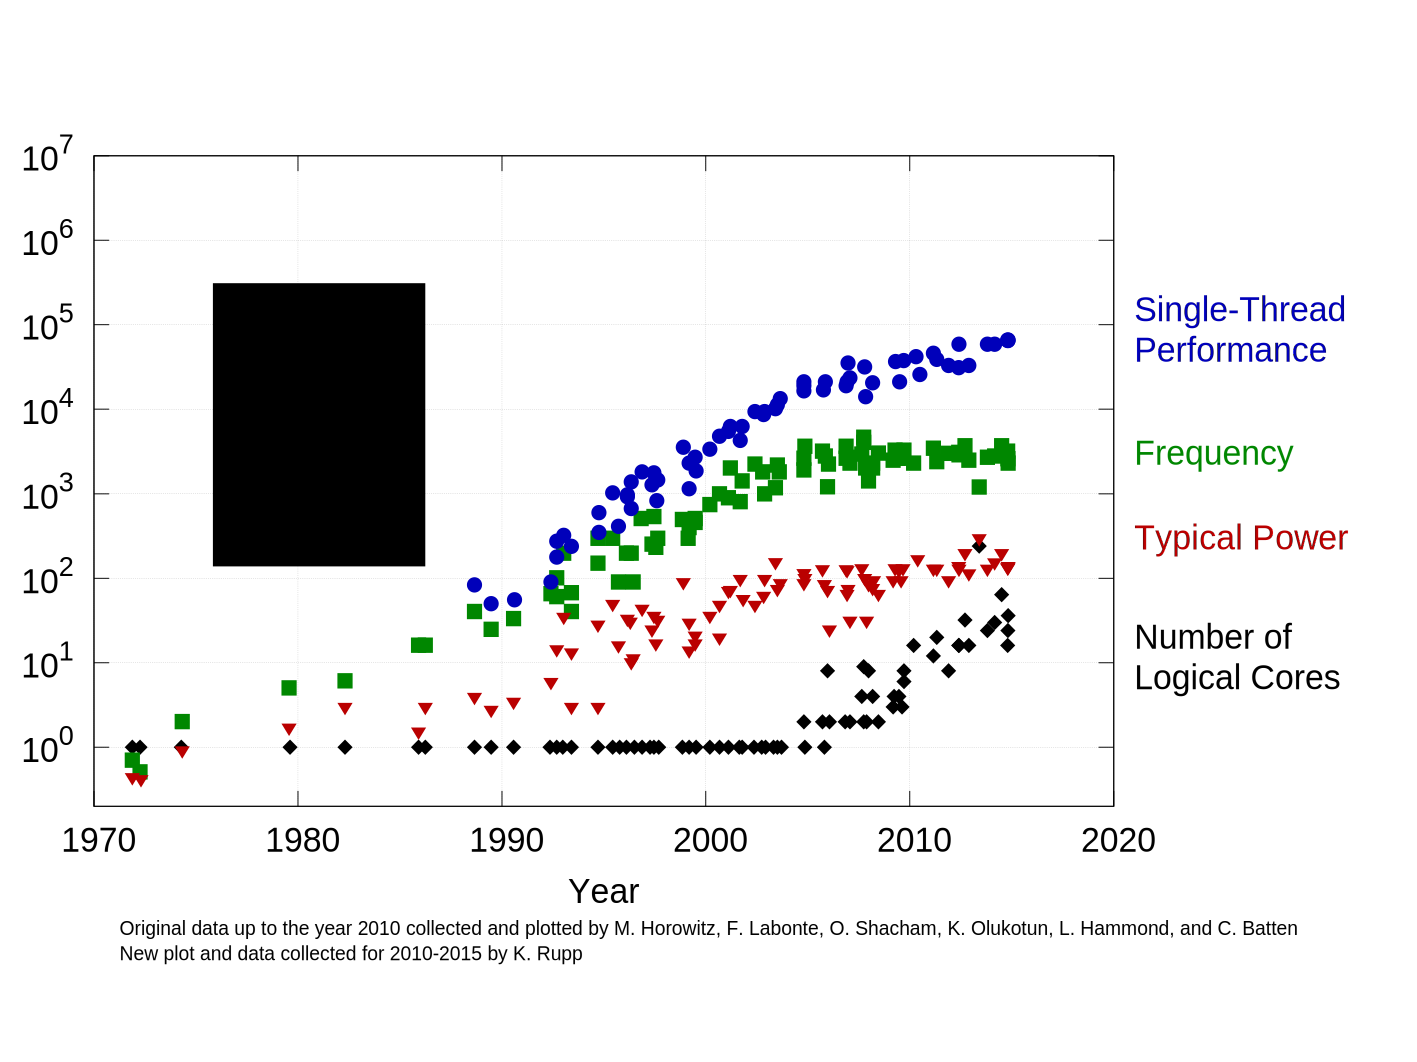
\includegraphics[scale=0.3]{fig/cpu}
  \end{center}
  \caption{CPU 발전 동향.}
  \label{fig:aim7}
\end{figure}

마지막 단계는 멀티코어이다.
그림 ~\ref{fig:aim7}과 같이 주파수는 계속 증가하다가, 2000년대 중반 멈추고, 그
때부터 코어수가 증가하고 있다. 
따라서 코어수가 100개 이상의 멀티코어 프로세서들도 등장함에 따라, 공유 때문에 야기하는 
새로운 문제가 발생하기 시작하였다.


\begin{figure}[h]
    \centering
    \includegraphics[width=0.6\textwidth]{fig/archcache}
    \caption{공유 메모리 시스템}
  \label{shared_memory}
\end{figure}

 
최근에 발생하는 문제들은 상당 부분이 캐시라인(cache-line)의 공유 때문에 발생하는 문제이고, 
이를 해결하기 위해서 최근에는 여러 운영체제(section~\ref{sec:osrelated}),
 락 기법(section~\ref{sec:lockrelated}), 그리고 자료구조와
 알고리즘(section~\ref{sec:datarelated})들이 개발되고 있다.

\begin{figure}[h]
    \centering
    \includegraphics[width=0.6\textwidth]{fig/archcache_percore}
    \caption{공유 메모리 시스템}
  \label{shared_memory}
\end{figure}

20년동안 싱글코어를 대상으로 연구가 되었고, 최근에는 이러한 문제를 해결하기 위해 
파티션닝 기법을 활용하여, 파티션닝 기법의 한 예로서는, 그림 x-x와 같이 공유되는 
전역 자료 구조를 각자 CPU에서 처리하도록 하는 방법이 있다.  
이러한 방법은 시스템 전반에 발생하는 캐시 커뮤니케이션 오버헤드를 줄일 수 있다. 

%$$$$$$$$$$$$$$$$$$$$$$$$$$$$$$$$$$$$$$$$$$$$$$$$$$$$$$$$$$$$$$$$$$$$$$$$$$$$$$$$
%Paragraph 1:Linux Scalability의 연구에 대한 설명
%$$$$$$$$$$$$$$$$$$$$$$$$$$$$$$$$$$$$$$$$$$$$$$$$$$$$$$$$$$$$$$$$$$$$$$$$$$$$$$$$

\newpage
\section{최근 운영체제 병렬화 연구}
\label{sec:osrelated}

%~\cite{Boyd-WickizerCorey}~\cite{Wentzlaff2010fOS}
%~\cite{Baumann2009Barrelfish}
%~\cite{Liu2009Tessellation}~\cite{Farrington2010Helios}

최근 병렬화 운영체제에 대한 연구는 새로운 확장성 있는 운영 체제를 만들거나 
기존 운영체제를 최적화 시키는 방향으로 연구가 진행되고 있다.
%~\cite{SilasBoydWickizer2010LinuxScales48}
%~\cite{AustinTClements2012RCUBalancedTrees}~\cite{Clements2013RadixVM}~\cite{SilasBoydWickizerPth}


\subsection{새로운 운영체제 제안}

\subsubsection{Corey}
Corey~\cite{Boyd-WickizerCorey}는 MIT의 PDOS(Parallel and Distributed Operating
Systems)에서 개발하였다.
Corey의 기본 철학은 커널 영역의 공유 데이터를 유저 응용프로그램이 사용할 수 있도록 인터페이스를 제공해서,
공유 데이터 때문에 발생하는 경합 문제를 유저 응용프로그램이 해결할 수 있도록 하는 것이다.
Corey가 이러한 방법을 사용한 이유는 코어 간의 캐시 일관성 작업 
때문에 성능이 저하되고, 이 현상이 발생하는 근본 원인이 운영체제가 응용프로그램의 특성에 관계 없이 
데이터를 공유하기 때문이다.
또한 하드웨어 역시 응용프로그램의 특성에 상관없이 캐시 메모리를 동기화 하는 방식을 사용하기 때문에,
기존 운영체제에서 취하는 방법을 사용하면 문제가 있다는 것이다. 
즉 기존 방법들은 매니코어 환경에서 응용프로그램 특성에 따라 최적화 할 수 없다는 문제점을 가진다. 
이러한 문제를 해결하기 위해, Corey는 응용프로그램의 워크로드에 따라 공유 문제를 응용프로그램 작성자가 
해결할 수 있는 방법을 제공해준다.
이러한 방법은 과거 연구되어온 커널의 자원을 유저와 공유할 수 있는 Exokernel~\cite{Engler1995EOS}의 개념을 가져와 
매니코어 시스템에 적용한 방법이며, Corey는 Exokernel과 같은 개념을 통해 확장성을 개선하였다.


\begin{figure}[h!]
    \centering
    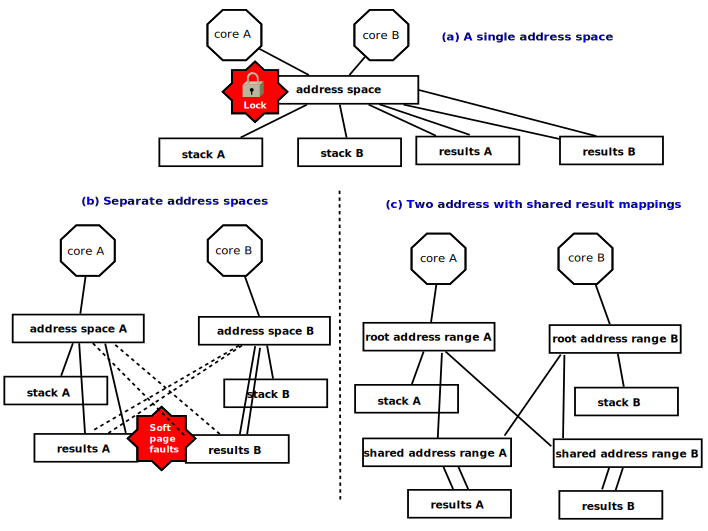
\includegraphics[width=1\textwidth]{fig/corey/corey}
    \caption{corey 운영체제 address space 공유 방법}
  \label{fig:corey}
\end{figure}

%$$$$$$$$$$$$$$$$$$$$$$$$$$$$$$$$$$$$$$$$$$$$$$$$$$$$$$$$$$$$$$$$$$$$$$$$$$$$$$$$
%Paragraph 2:Corey의 3가지 기본 개념 설명
%$$$$$$$$$$$$$$$$$$$$$$$$$$$$$$$$$$$$$$$$$$$$$$$$$$$$$$$$$$$$$$$$$$$$$$$$$$$$$$$$
Corey는 3가지 기본적인 개념(Address Rages, Kernel Core, Shares)을 가지고 있다. 
첫째, Address Rages는 운영체제에서 여러 스레드간의 공유하는 데이터인 Address Space에 대해서 다룬다.
대부분의 운영체제는 Address Space를 그림~\ref{fig:corey}(a)와 같이 Single Address Space로
구성하는 경우와 그림~\ref{fig:corey}(b)와 같이 퍼코어 기반의 Separate Address Space로 구성하는 경우가
있다. 
만약 Single Address Space를 사용할 경우 모든 코어가 같은 Address Space를 사용함에 따라 반드시 락이
필요하고 이 락 때문에 스레드들이 직렬화된다.
예를 들어, 맵리듀스(MapReduce)와 같은 응용프로그램을 사용할 경우 맵 단계에서 굉장히 많은 락 경합이 발생하게 된다.
또한, 만약 Separate Address Space를 사용할 경우 리듀스 단계에서 공유하지 않은 데이터에 접급함에 따라 
소프트 페이지 폴트(Soft Page Fault)가 많이 발생하는 문제가 있다.
Corey는 이러한 문제를 Address Rages라는 새로운 개념으로 해결하였다. 
이것은 그림~\ref{fig:corey}(c)와 같이 Separate Address Space를 제공함과 동시에 중간 결과를 공유할 수 있는
방법을 제공함으로 Single Address Space의 장점을 동시에 취한다.
다음으로, Kernel Core는 응용프로그램을 공유 메모리를 사용하지 않고, 특정 코어에 
독점 할당 시켜주고 공유는 IPC로 하도록 제공하는 기술이다. 
따라서 스케줄러와 인터럽트에 방해를 받지 않고 캐시 지역성을 높여 성능을 향상 시키는 방법이다.
마지막으로, 공유는 Exokernel과 같이 어떻게 커널 자료구조를 접근할 수 있는 지에 대해서 기능을 제공해준다.


\subsubsection{Barrelfish}

%$$$$$$$$$$$$$$$$$$$$$$$$$$$$$$$$$$$$$$$$$$$$$$$$$$$$$$$$$$$$$$$$$$$$$$$$$$$$$$$$
%Paragraph : Barrelfish의 특징 설명
%$$$$$$$$$$$$$$$$$$$$$$$$$$$$$$$$$$$$$$$$$$$$$$$$$$$$$$$$$$$$$$$$$$$$$$$$$$$$$$$$
Barrelfish~\cite{Baumann2009Barrelfish}는 취히리의 ETH와 마이크로 소프트(Microsoft)가
공동 연구하여 만든 운영체제이다.
Barrelfish는 멀티커널(Multikernel) 운영체제 중 하나 이고, 기본적인 철학은 공유 메모리 시스템 
기능들을 분산 처리 방식으로 구현하자는 것이다.
예를 들어, 운영체제에서 각 코어는 네트워크로 분산 된 시스템으로 가정하고, 서로 다른 코어 간에는 메시지 
패싱을 통해 통신을 하여 성능을 향상 시킨 방법이다. 
이러한 방법을 사용한 이유는 캐시 구조로 된 시스템의 단일화된 인터커넥트가 코어가 증가할 수록 캐시 
일관성 트래픽 문제를 야기 하기 때문에, 하나의 인터커넥트를 이용하는 하드웨어 캐시 일관성 
프로토콜을 사용하는 방법보다 메시지 패싱 방법이 오히려 더 높은 성능을 보이기 때문이다. 

%$$$$$$$$$$$$$$$$$$$$$$$$$$$$$$$$$$$$$$$$$$$$$$$$$$$$$$$$$$$$$$$$$$$$$$$$$$$$$$$$
%Paragraph : Barrelfish의 구조 설명 
%$$$$$$$$$$$$$$$$$$$$$$$$$$$$$$$$$$$$$$$$$$$$$$$$$$$$$$$$$$$$$$$$$$$$$$$$$$$$$$$$
이러한 Barrelfish의 구현은 그림~\ref{fig:Barrelfish}과 같다.
커널 레벨에서는 하드웨어와 밀접한 CPU Driver가 하드웨어 인터페이스를 제공한다.
CPU Driver는 유저 레벨의 모니터(Monitor)와 함께 하나의 운영체제 처럼 동작하며, 
이것은 각 코어에 하나의 운영체제가 동작하는 것 처럼 보이는 멀티커널(Multikernel)의 구조를 가진다. 
응용프로그램은 여러 코어를 이용할 수 있는데, 이러한 환경을 제공하기 위해 존재하는 것이 모니터이다. 
모니터는 운영체제의 기본 기능을 제공하기 위해 존재하며, 공유 메모리를 사용하기 
보다는 복제(Replication)와 IPC와 같은 분산 시스템에서 사용하는 방법을 사용한다. 
모니터는 View라는 상태를 가지고 복제를 수행한다. 
이러한 방법 역시 분산 시스템에서 사용하는 방식과 같이 시스템을 구성하여, 캐시 커뮤니케이션 때문에 발생하는 
시스템의 인터커넥트의 로드를 줄일 수 있다.

\begin{figure}[h!]
    \centering
    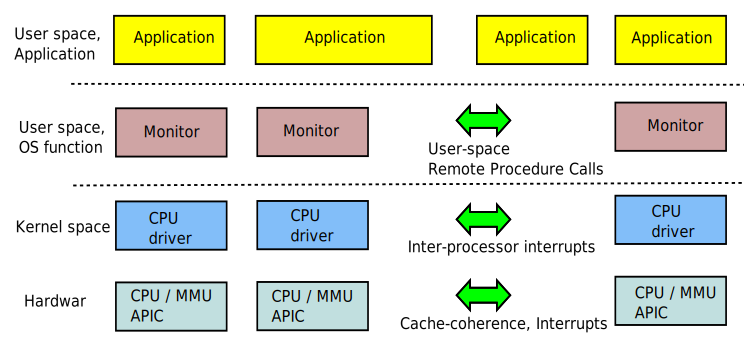
\includegraphics[width=1\textwidth]{fig/multikernel/multikernel}
    \caption{Barrelfish 구조}
  \label{fig:Barrelfish}
\end{figure}

%$$$$$$$$$$$$$$$$$$$$$$$$$$$$$$$$$$$$$$$$$$$$$$$$$$$$$$$$$$$$$$$$$$$$$$$$$$$$$$$$
%Paragraph : Barrelfish의 구조의 단점
%$$$$$$$$$$$$$$$$$$$$$$$$$$$$$$$$$$$$$$$$$$$$$$$$$$$$$$$$$$$$$$$$$$$$$$$$$$$$$$$$
Barrelfish의 단점으로는 Barrelfish의 구조적인 철학이 공유를 최대한 줄이는 것인데, 
이것은 결국 로드 밸런싱을 수행할 수 없는 단점을 가진다. 
예를 들어 하나의 코어에 많은 스레드들이 같이 돌고 있고, 다른 코어에는 아무런 
스레드도 없는 경우, Barrelfish는 분산 시스템 처럼 수행되므로 동적으로 스레드에 대한 정보들을 
다른 코어로 전송할 수가 없는 문제점을 가진다.
즉 분산 시스템의 전형적인 단점인 로드 밸런싱이 어려우므로 응용프로그램에 따라,
로드가 한 쪽에 몰리는 경우, 느려진 코어의 스레드들을 기다려야 하기 때문에 전체적인 
성능이 저하된다.  

\subsubsection{FusedOS}
%$$$$$$$$$$$$$$$$$$$$$$$$$$$$$$$$$$$$$$$$$$$$$$$$$$$$$$$$$$$$$$$$$$$$$$$$$$$$$$$$
%Paragraph : Fused OS의 특징 설명
%$$$$$$$$$$$$$$$$$$$$$$$$$$$$$$$$$$$$$$$$$$$$$$$$$$$$$$$$$$$$$$$$$$$$$$$$$$$$$$$$
FusedOS는 IBM 연구소에서 개발되었으며, 모노리틱 구조와 마이크로 구조의 장점을 이용한 운영체제이다.
FusedOS 운영체제는 기존 연구들은 모두 경량 커널(LWK: Light-Weight Kernel) 또는 정량 커널(FWK:
Full-Weight Kernel) 둘 중 하나의 방식으로만 개발되었으나, 최초로 LWK와 FWK를 
혼합하여 만든 운영체제이다.
혼합하여 만든 운영체제인 FusedOS의 장점은 LWK를 통하여 FWK이 가지고 있는 근본적인 확장성 
문제를 해결할 수 있다는 것과, 과학에서 많이 사용되는 특정한 목적으로 개발된 응용프로그램을 
LWK에서 동작시킴에 따라 커널의 간섭이 없이 동작 시킬 수 있다는 것이다. 
또한 LWK의 장점 뿐만 아니라, FWK의 장점 중 하나인 리눅스로 인하여 기존 만들어진 라이브러리들을 
리눅스의 장점을 모두 활용 할 수 있기 때문이다.
 
\begin{figure}[h!]
    \centering
    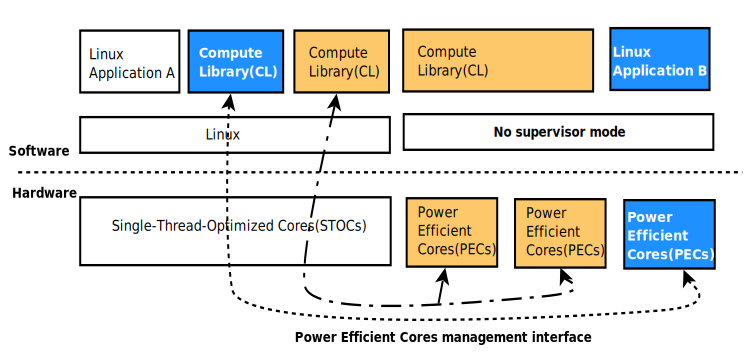
\includegraphics[width=1\textwidth]{fig/fusedos/fusedos}
    \caption{FusedOS 구조}
  \label{fig:FusedOS}
\end{figure}

%$$$$$$$$$$$$$$$$$$$$$$$$$$$$$$$$$$$$$$$$$$$$$$$$$$$$$$$$$$$$$$$$$$$$$$$$$$$$$$$$
%Paragraph : Fused OS의 구조 설명
%$$$$$$$$$$$$$$$$$$$$$$$$$$$$$$$$$$$$$$$$$$$$$$$$$$$$$$$$$$$$$$$$$$$$$$$$$$$$$$$$
이러한 FusedOS의 구조는 그림~\ref{fig:FusedOS}과 같다. 
그림과 같이 FusedOS의 하드웨어는 성능 좋은 코어 그룹(STOCs: Single-Thread-Optimized Cores)과
전력에 효율적인 코어 그룹(PECs: Power Efficient Cores)으로 구성되어 있다.
PEC는 STOC의 기능 중 하나이고 관리자(Supervisor) 모드를 포함하고 있지는 않는다. 
STOC에는 리눅스 운영체제가 동작하고, 리눅스에 기능을 추가하여 Compute Library(CL)이 PEC에 
접근이 가능하도록 설계되었다.

CL은 마치 리눅스 응용프로그램으로 동작하며, 실행이 되면 다음으로 가벼운 커널을 PEC 메모리에 
전달하고 그 후 가벼운 커널은 PEC코어에서 동작하게 된다.
이러한 구조를 통해, HPC 응용의 성능을 보여주면서 리눅스 운영체제의 기능을 제공할 수 있는 장점을 가진다. 
FusedOS의 성능은 HPC 운영체제 코어와 연산을 위한 코어가 분리되었기 때문에, 운영체제의 
방해를 받지 않아 기존 리눅스보다 높은 성능을 보인다.
이것을 통해 기존 운영체제의 병목 현상인 캐시 일관성 유지 때문에 발생하는 확장성 문제를 해결할 수 있다.
하지만 FusedOS의 문제점은 독립적으로 코어에 LWK를 할당하여 호출하는 방법을 사용하므로,  
응용프로그램을 실행하고 종료하는데 추가적인 시간이 필요한 단점을 가진다.

\subsection{기존 운영체제 최적화}

\subsubsection{Linux Scalability}

앞에서 설명한 새로운 운영체제에 대한 연구 뿐만 아니라 기존 운영체제의 확장성에 대한 연구가 진행되었다. 
특히 MIT PDOS 연구 그룹은 새로운 운영체제가 아닌 리눅스 커널을 대상으로 매니코어 환경에서 확장성을 연구하였다.
실제 많이 사용되는 7가지의 응용프로그램(Exim, Memcached, Apache, PostgreSQL, Gmake, Psearchy,
MapReduce)을 가지고 MOSBENCH라는 응용프로그램 벤치마크를 만들어 리눅스 커널을 대상으로 실험을 
하였고, 측정 중 발생되는 여러 문제를 해결하여, 리눅스 커널의 확장성을 향상시켰다.

\begin{figure}[h!]
    \centering
    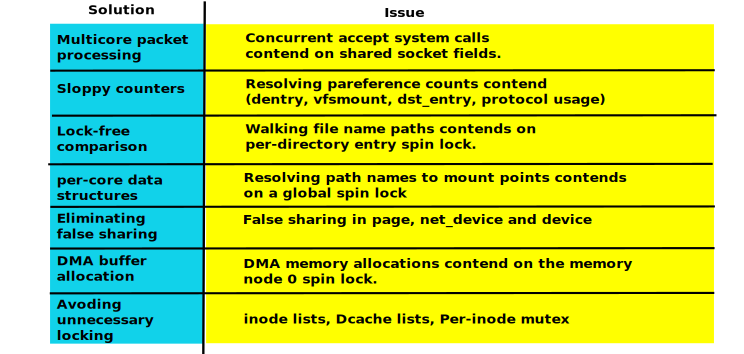
\includegraphics[width=1\textwidth]{fig/linux/linux}
    \caption{linux scalability 분석 연구}
  \label{fig:linux}
\end{figure}

이 연구는 그림~\ref{fig:linux}와 같이 총 7가지의 기술을 활용하였고, 추가적으로 응용프로그램을 직접 수정하여 
커널의 확장성을 개선하였다.
먼저 7가지 기술 중 하나는 멀티코어 패킷 프로세싱이 있다. 
그 동안 리눅스 커널은 네트워크 멀티코어 패킷을 위해 멀티 큐를 사용하여 성능과 확장성을 이루었으나, 
만약 클라이언트 연결 주기가 짧을 경우 이러한 방법도 역시 성능과 확장성 문제를 가진다.
따라서 이 연구 그룹은 동시 다발 적으로 연결을 요청하는 아파치(Apache) 응용프로그램과 같은 경우 
퍼코어 큐에 저장하도록 커널의 소켓 함수 중 \code{accpet()}을 수정하였다. 
이 것은 싱글 리스닝(Listening) 소켓을 보호하기 위해 존재하는 락을 제거할 수 있어 확장성을 향상 시킨다.

다음으로 이 연구 그룹은 리눅스의 참조 카운터 때문에 발생하는 캐시 일관성 트래픽을 제거하기 위해
\textit{sloppy counter}를 만들었다. 
디렉터리 엔트리 오브젝트(\code{dentrys}), 마운트된 파일 시스템 오브젝트(\code{vfsmounts}) 그리고 
네트워크 프로토콜에서의 메모리 할당을 추적하기 위한 전역 변수들을 모두 \textit{sloppy counter}로 수정하여 
성능을 향상 시켰다.
또한 리눅스 커널은 디렉토리 엔트리 캐시의 이름을 찾는 부분에 \textit{per-dentry spin lock} 때문에 문제가
존재하였다.
이 문제를 해결하기 위해 연구 그룹은 리눅스의 \textit{lock-free page-cache lookup protocol}과
유사한 방법을 활용하여 문제가 발생하는 전역 \textit{spin lock}을 제거하였다.
그 이외에도 퍼코어 방법을 사용한 방법과 캐시 라인의 \textit{false sharing} 때문에 발생하는 성능 저하 문제, 
이더넷 디바이스 DMA 버퍼가 한쪽 노드에만 할당되어 발생하는 확장성 문제와 그리고 불필요한 락을 
제거하여 리눅스 커널의 확장성을 향상 시켰다.  

\subsubsection{BonsaiVM}
%$$$$$$$$$$$$$$$$$$$$$$$$$$$$$$$$$$$$$$$$$$$$$$$$$$$$$$$$$$$$$$$$$$$$$$$$$$$$$$$$
%Paragraph : BonsaiVM 특징 설명
%$$$$$$$$$$$$$$$$$$$$$$$$$$$$$$$$$$$$$$$$$$$$$$$$$$$$$$$$$$$$$$$$$$$$$$$$$$$$$$$$
BonsaiVM은 MIT PDOS에서 개발한 리눅스 커널을 위한 가상 메모리 관리 시스템이다. 
리눅스의 멀티 스레드들은 하나의 Address Space를 공유하게 되는데, 이러한 공유된 Address Space을 사용하는 
스레드들은 \code{mmap/munmap}과 소프트 페이지 폴트간에 락 경합이 발생된다.
리눅스는 공유된 Address Space를 보호하기 위해, 락 경합 중 블락킹 동기화 기법 중 하나인
읽기-쓰기(reader-writer) 세마포어를 사용하여 보호한다.
이러한 동기화 기법을 사용함에 따라, Address Space를 때문에 여러 스레드들이 블록이 걸리는 현상이 많이 발생하는데, 
이 때문에 결국 코어가 많아져서 여러 스레드가 같은 Address Space에 접근하면 Single Address Space 때문에 성능이
저하되는 문제가 발생한다.

\begin{figure}[h!]
    \centering
    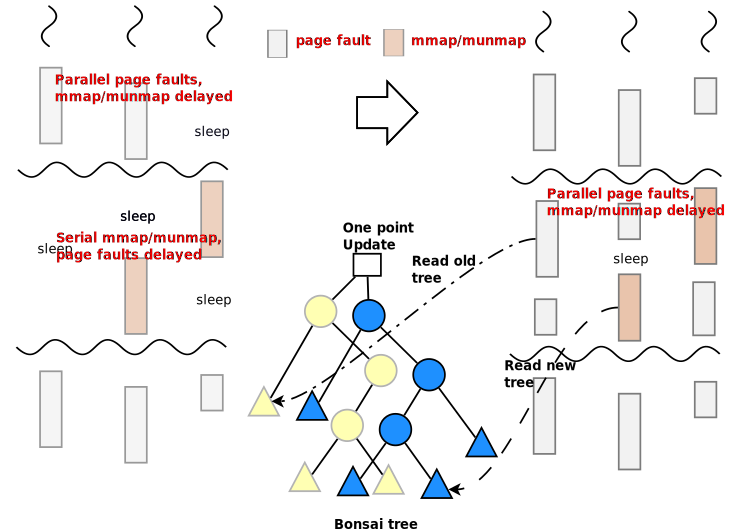
\includegraphics[width=1\textwidth]{fig/bosaivm/bosaivm}
    \caption{Address space 문제와 BosaiVM을 이용한 해결}
  \label{fig:bonsaivm}
\end{figure}

그림~\ref{fig:bonsaivm}의 왼쪽 부분은 이러한 Address Space를 문제를 보여준다. 
병렬로 수행이 가능한 페이지 폴트 때문에 \code{mmap/munmap} 함수는 블록이 걸리고, 병렬로 
수행이 불가능한 \code{mmap/munmap} 함수가 수행되면, \code{mmap/munmap} 함수 뿐만 아니라 
페이지 폴트까지 블록에 걸린다.
이러한 Single Address Space 문제를 해결하기 위해, 앞에서 설명한 Corey 운영체제와 같이 새로운 운영체제를 
만드는 등 여러 연구들이 진행되었지만, 이 연구에서는 새로운 운영체제가 아닌 기존 리눅스 커널을 대상으로 
동기화 기법 중 하나인 RCU와 새로운 밸런스 트리(\code{Bonsai})를 이용하여 Single Address Space 문제를
해결하였다.
즉 리눅스 커널을 대상으로 개선한 연구이며, 
리눅스 커널 중 상당히 복잡한 가상 메모리 시스템에 직접 RCU라는 동기화 기법을 사용하여, 
성능 확장성을 향상 시킨 연구이다.
 
BonsaiVM은 총 3가지 기법(\textit{fault locking, hybrid locking/RCU, pure RCU})을 통해
Single Address Space 문제를 해결하였다.
이 중 앞의 두 가지 방법은 리눅스 커널의 구현 의존 적인 해결 방법이고, \textit{pure RCU}는 
기존 리눅스 커널의 레드-블랙 트리를 사용하지 않고 RCU를 사용할 수 있는 
새로운 \code{Bonsai} 트리 자료구조를 만들어 문제를 해결한 방법이다. 
\code{Bonsai} 트리는 그림~\ref{fig:bonsaivm}과 같이 이진 트리로 구성되어 있다. 
\code{Bonsai} 트리의 가장 큰 특징은 루트 노드의 업데이트가 원자적 명령으로 한번에 이루어 진다는 것이다. 
그 이유는 Bonsai 트리는 함수형 트리 형식으로 개발되어서, 밸런스를 수행하는 동안에도 읽기 연산들은 
오래된 트리의 값을 읽으며 병렬로 수행할 수 있는 장점을 가진다는 것이다.
즉 RCU의 장점을 활용하여 여러 읽기 연산과 한가지의 쓰기 연산을 수행하는 스레드들이 병렬로 수행할 수 
있는 장점을 가진다. 
하지만 여러 스레들간에 경쟁이 발생하지 않는 경우, 트리 검색이 기존 레드-블랙 트리에 비해 많은 성능 
오버헤드가 존재하는 문제점이 있다. 
 
%$$$$$$$$$$$$$$$$$$$$$$$$$$$$$$$$$$$$$$$$$$$$$$$$$$$$$$$$$$$$$$$$$$$$$$$$$$$$$$$$
%Paragraph 2: 기법 설명
%$$$$$$$$$$$$$$$$$$$$$$$$$$$$$$$$$$$$$$$$$$$$$$$$$$$$$$$$$$$$$$$$$$$$$$$$$$$$$$$$

\subsubsection{RadixVM}

%$$$$$$$$$$$$$$$$$$$$$$$$$$$$$$$$$$$$$$$$$$$$$$$$$$$$$$$$$$$$$$$$$$$$$$$$$$$$$$$$
%Paragraph : RadixVM 특징 설명
%$$$$$$$$$$$$$$$$$$$$$$$$$$$$$$$$$$$$$$$$$$$$$$$$$$$$$$$$$$$$$$$$$$$$$$$$$$$$$$$$
RadixVM은 BosaiVM과 같은 연구 그룹이 수행한 연구이며, 
Single Address Space 때문에 발생하는 확장성 문제를 해결하기 위해, 연구 용 운영체제인 sv6의 가상 메모리에 
대한 부분을 수정하여 Single Address Space 문제를 해결한 연구이다.
그 이유는 리눅스의 가상 메모리를 수정하는 것은 굉장히 복잡하여 리눅스 커널에 직접 적용하기 힘든 문제점이 
있기 때문에, 상대적으로 덜 복잡한 sv6 운영체제에 새로운 개념인 RadixVM을 적용하였다. 
RadixVM은 BonsaiVM과 같이 가상 메모리 시스템에서 공유되는 Address Space가 \code{mmap, unmap, page
fault} 함수 들로 인해 서로 경쟁함으로 발생하는 문제를 3가지 접근을 통해 해결하였다. 

\begin{figure}[h!]
    \centering
    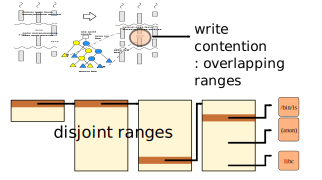
\includegraphics[width=1\textwidth]{fig/radix/radix}
    \caption{RadixVM의 해결 방법}
  \label{fig:radix}
\end{figure}

%$$$$$$$$$$$$$$$$$$$$$$$$$$$$$$$$$$$$$$$$$$$$$$$$$$$$$$$$$$$$$$$$$$$$$$$$$$$$$$$$
%Paragraph : RadixVM  기법 설명 - 1
%$$$$$$$$$$$$$$$$$$$$$$$$$$$$$$$$$$$$$$$$$$$$$$$$$$$$$$$$$$$$$$$$$$$$$$$$$$$$$$$$
첫째, 기존 밸런스 트리를 사용하지 않고, \code{radix} 트리를 이용하는 것이다. 
그 이유는 RadixVM의 궁극적인 목적은 가상 메모리와 관련된 연산에 대해서는 최대한 공유를 피하자는 것인데, 
실제로 모든 메모리 맵을 배열로서 만들면 모든 가상 메모리 관련 연산들의 충돌은 일어나지 않는다. 
하지만 단순히 배열을 이용한 방법은 너무 많은 메모리 사용량이 요구된다.
따라서 메모리 오버헤드 문제를 해결하기 위한 가장 좋은 방법은 하드웨어 페이지 테이블처럼 동작하는 
배열과 가장 비슷한 기수(Radix) 트리를 이용하는 것이 이 연구의 핵심 내용이다. 
이처럼 기수 트리는 트리의 읽기와 쓰기 연산을 메모리의 서로 다른 부분에 접근하도록 만들어 준다.
따라서 배열을 사용한 방법과 같이 충돌 없이 사용 가능함과 동시에 메모리 오버헤드도 줄인다. 
결론적으로 여러 스레들이 접근 할 수 있을 뿐 만아니라 메모리 사용량도 밸런스 트리와 비슷한 
수준을 유지 할 수 있는 장점을 가진다.

%$$$$$$$$$$$$$$$$$$$$$$$$$$$$$$$$$$$$$$$$$$$$$$$$$$$$$$$$$$$$$$$$$$$$$$$$$$$$$$$$
%Paragraph : RadixVM  기법 설명 - 2
%$$$$$$$$$$$$$$$$$$$$$$$$$$$$$$$$$$$$$$$$$$$$$$$$$$$$$$$$$$$$$$$$$$$$$$$$$$$$$$$
\code{RadixVM}의 두번째 기법은 \code{munmap}할 때 발생하는 \textit{TLB shutdown} 문제를 해결한
방법이다.
이러한 \textit{TLB shutdown} 문제가 발생하는 이유는 \code{unmap} 함수는 반드시 어떠한 코어의 페이지도 매핑이 
안된 상태로 끝나야 하는데, 이를 유지하기 위해 \code{unmap} 함수는 모든 코어에 \textit{TLB shutdonw} 메시지를
남기며, 이것이 바로 코어가 증가 할 수록 불필요하게 모든 코어에 \textit{TLB shutdown} 메시지를 발생 시키므로 
성능 문제를 야기 시킨다.
\code{RadixVM}에서는 이러한 \textit{TLB shutdown} 문제를 퍼코어 페이지 테이블을 이용하여 해결하였다. 

%$$$$$$$$$$$$$$$$$$$$$$$$$$$$$$$$$$$$$$$$$$$$$$$$$$$$$$$$$$$$$$$$$$$$$$$$$$$$$$$$
%Paragraph : RadixVM  기법 설명 - 2
%$$$$$$$$$$$$$$$$$$$$$$$$$$$$$$$$$$$$$$$$$$$$$$$$$$$$$$$$$$$$$$$$$$$$$$$$$$$$$$$
\code{RadixVM}의 마지막 기법은 새로운 \code{refcache}라는 레퍼런스 카운터(Reference Counter)를 제공한다는
것이다.
실제 운영체제에서 레퍼런스 카운터는 최근 운영체제의 가장 큰 확장성 저해요소 중에 하나로 본다.
그 이유는 레퍼런스 카운터는 많은 캐시 일관성 트래픽을 발생 시키기 때문이다.
이러한 레퍼런스 카운터는 기본적으로 3가지 종류로 개발되고 있다. 
먼저 가장 쉬운 방법인 락을 이용하는 방법이 있다. 
즉 모든 증가/감소 명령의 앞뒤에 락을 호출하는 것이다. 
이것은 락 때문에(락 자체가 전변 변수를 이용) 상당히 많은 캐시-라인 경합이 발생된다. 
다른 방법으로는 원자적 증가/감소 명령을 이용하는 것이다. 
하지만 이러한 방법도 결국 전역 변수 때문에 캐시-라인 경합이 발생한다. 
최근의 방법으로는 파티션닝 기법 중 하나인 퍼코어 카운터를 이용하는 것이다. 
하지만, 단순히 퍼코어 카운터를 이용하는 것은 코어 수에 비례하여 공간에 대한 오버헤드를 가지게 된다.
\code{RadixVM}은 이러한 확장성과 메모리 사용량에 대한 오버헤드를 동시에 줄이기 위해, 
특정 시간(Epoch, 10ms)을 기반으로 퍼코어에 저장된 델타 카운트를 
주기적으로 체크하여 퍼코어에 저장된 카운터의 상태를 보고 전역 카운터에 적용하는 방법을 사용하였다.
이 방법은 확장성을 늘릴 수 있을 뿐만 아니라, 동시에 공간에 대한 오버헤드를 줄인다. 

\subsubsection{Scalable Commutativity Rule}

%$$$$$$$$$$$$$$$$$$$$$$$$$$$$$$$$$$$$$$$$$$$$$$$$$$$$$$$$$$$$$$$$$$$$$$$$$$$$$$$$
%Paragraph : SC rule 특징 및 역사 설명 
%$$$$$$$$$$$$$$$$$$$$$$$$$$$$$$$$$$$$$$$$$$$$$$$$$$$$$$$$$$$$$$$$$$$$$$$$$$$$$$$$
SC Rule(Scalable Commutativity Rule)은 MIT PDOS 연구 그룹에서 운영체제의 확장성 개선을 위해 새로운
관점으로 바라본 연구이다.
기존 연구들은 대부분 운영체제의 병목지점을 추출한 후 발견된 병목지점을 해결하기 위해 새로운 
동기화 기법을 개발하거나 기존 개발된 동기화 기법을 적용하는 방법을 사용했다. 
하지만, 이러한 방법들은 모두 워크로드가 다름에 따라 서로 다른 양상을 가지고, 
또한 문제를 해결하는데 너무 오랜 시간이 걸리는 문제점을 가지고 있다.
실제 확장성에 대한 문제는, 대부분 설계 단계에서 해결이 가능하며, 인터페이스를 확장성 있게 설계하면 
확장성 있는 시스템을 만들 수 있다는 것이다.
그 이유는 기존 개발되어온 운영체제(예를 들어 리눅스)는 응용프로그램이 커널의 자원을 
확장성 있게 사용하면 확장성에 문제가 없기 때문이다. 
따라서, 확장성 있는 설계가 중요하며 이를 위해 리눅스 시스템 콜 연산에 대한 가환성(Commutativity)을 정의하였고, 
그에 대한 이론을 설명한 논문이다.
가환성을 예를 들어 설명하면, 원자적으로 값 X를 변수 A에 추가하고, 
다른 CPU가 원자적으로 같은 변수에 Y라는 값을 추가하였다면, 
두 가지의 명령의 순서는 상관 없고, 결국에는 X + Y의 값이 변수 A에 저장된다는 것이다.
이러한 수학적인 가환성을 리눅스의 시스템 콜을 대상으로 새로운 가환성을 정의 하였다.

%$$$$$$$$$$$$$$$$$$$$$$$$$$$$$$$$$$$$$$$$$$$$$$$$$$$$$$$$$$$$$$$$$$$$$$$$$$$$$$$$
%Paragraph : SC rule 예제 설명 
%$$$$$$$$$$$$$$$$$$$$$$$$$$$$$$$$$$$$$$$$$$$$$$$$$$$$$$$$$$$$$$$$$$$$$$$$$$$$$$$$
저자는 SIM(State-dependent, Interface-based, Monotonic)라고 부르는 새로운
POSIX 운영체제의 가환성(commutativity)에 대해서 정의를 하였다.
또한 POSIX의 오퍼레이션에 대해서 가환성을 여러 오퍼레이션을 예를 들어 설명하였다.
\code{open(``a'', O\_CREAT|O\_EXCL)}을 두 개의 코어가 같은 디렉토리에서 수행하면 가환성이 없는데, 
이것을 다른 디렉토리에서 수행하면 가환성을 가진다는 것이다.
저자가 주장하는 SIM 가환성은 이러한 시스템 콜 함수들을 구별할 수 있게 만들어주고, 결국 
인터페이스 레벨에서 가환성을 가짐에 따라 확장성 있는 시스템을 가질 수 있다는 것이다.  
또 다른 예로 프로세스를 복사하는 \code{fork()}는 가환성을 가지고 있지 않는데, 
\code{fork()}를 \code{posix\_spawn()}으로 수정하면 가환성을 가지게 되고, 이것은 결국 
확장성을 향상 시키게 된다. 
이러한 원리는 결국 앞에서 설명하였듯이, 리눅스는 응용프로그램의 방법에 따라 확장성을 가질 수 있는데 
이 연구는 리눅스 특성들을 잘 이용한 연구이다. 
결국 리눅스 커널은 가환성을 잘 지키도록 호출 해주면, 확장성을 향상 시킬 수 있고 
이것은 설계 단계에서 처리할 수 있다는 것이다.
또한 저자는 QEMU을 수정하여 리눅스의 가환성을 분석 할 수 있는 \code{Commuter}라는 툴을 제공한다. 
이러한 툴을 통해 설계 단계에서 확장성 문제를 발견할 수 있으며, 이 툴을 통해 기존 운영체제(리눅스, sv6)의 
문제점을 분석하였다. 


%$$$$$$$$$$$$$$$$$$$$$$$$$$$$$$$$$$$$$$$$$$$$$$$$$$$$$$$$$$$$$$$$$$$$$$$$$$$$$$$$
%Paragraph 3: Scalable Data Structure and Lock에 대한 연구
%$$$$$$$$$$$$$$$$$$$$$$$$$$$$$$$$$$$$$$$$$$$$$$$$$$$$$$$$$$$$$$$$$$$$$$$$$$$$$$$$
\newpage
\section{확장성 있는 락 연구}
\label{sec:lockrelated}
%Scalable locks have been designed by the
%queue-based locks~\cite{MellorCrummey1991MCS}~\cite{Magnusson1994QLC},
%~\cite{Wang2016BeMyGuest},
%~\cite{Scott2013SS}
%~\cite{Bueso2014MCS}~\cite{Bueso2015STP}
%hierarchical locks~\cite{Radovic2003HBL}~\cite{Chabbi2016CLL} and
%~\cite{Luchangco2006HCQ}
%~\cite{Chabbi2015HPL}
%delegation
% techniques~\cite{Hendler2010FC}~\cite{Fatourou2012RCS}~\cite{Delegation2014}.

%Scalable locks have been designed by the
%queue-based locks~\cite{MellorCrummey1991MCS}~\cite{Magnusson1994QLC},
%~\cite{Wang2016BeMyGuest},
%~\cite{Scott2013SS}
%~\cite{Bueso2014MCS}~\cite{Bueso2015STP}
%hierarchical locks~\cite{Radovic2003HBL}~\cite{Chabbi2016CLL} and
%~\cite{Luchangco2006HCQ}
%~\cite{Chabbi2015HPL}
% delegation
%techniques~\cite{Hendler2010FC}~\cite{Fatourou2012RCS}~\cite{Delegation2014}.
확장성 있는 락들은 큐 기반의 락~\cite{MellorCrummey1991MCS}~\cite{Magnusson1994QLC},
~\cite{Wang2016BeMyGuest},
~\cite{Scott2013SS}
~\cite{Bueso2014MCS}~\cite{Bueso2015STP}과 계층적 락~\cite{Radovic2003HBL}~\cite{Chabbi2016CLL} and
~\cite{Luchangco2006HCQ}
~\cite{Chabbi2015HPL} 그리고 위임하는 방법(delegation
techniques)~\cite{Hendler2010FC}~\cite{Fatourou2012RCS}~\cite{Delegation2014}을 사용한다.

%Some approaches have been gradually adapted in real production software.
%For example, Linux kernel has replaced non-scalable locks with
%MCS locks~\cite{overviewofkernellock}.
%Our research is similar to the delegation techniques because
%the \LDU's \code{synchronize} function runs as a
%combiner thread;it improves cache locality.

\subsection{큐 기반의 락(Queued Lock)}


\subsubsection{MCS}



\subsection{계층적 락}

이 중 우리의 연구는 LDU의 \code{synchronize} 함수가 마치 FC의 컴파이너 쓰레드(combiner thread)와 같이
동작함으로 위임하는 방법과 비슷하다. 이것은 캐시의 지역성을 높이는 방법이다.
%However, our approach not only can improve cache locality but also
%can eliminate synchronization methods during updates due to using a lock-free
% manner.
하지만, 우리의 방법은 캐시의 지역성을 높일 뿐만아니라 업데이트 명령을
 수행하는 동안 락 프리(lock-free) 방법으로 동기화 기법들을 제거 할 수 있다. 
%MCS~\cite{MellorCrummey91}, a scalable lock.
%, is used in the Linux
%.
%In read-mostly data structures, RCU~\cite{McKenney98} can be quite useful.
%However, 
\subsubsection{HBL}



\subsubsection{CLL}


\subsubsection{HCQ}



\subsection{Delegation techniques}

\subsubsection{Flat Combining}



\subsubsection{OpLog}

OpLog는 RCU와 반대로 업데이트 비율이 높은 업데이트 헤비(Update heavy)한 자료구조를 위해 만든 
동기화 기법 중 하나이다.


\begin{figure}[h]
    \centering
    \includegraphics[width=0.8\textwidth]{fig/oplog_log}
    \caption{OpLog의 업데이트 방법}
  \label{fig:oplog}
\end{figure}





%$$$$$$$$$$$$$$$$$$$$$$$$$$$$$$$$$$$$$$$$$$$$$$$$$$$$$$$$$$$$$$$$$$$$$$$$$$$$$$$$
%Paragraph 2:Concurrent updates에 대한 연구
%$$$$$$$$$$$$$$$$$$$$$$$$$$$$$$$$$$$$$$$$$$$$$$$$$$$$$$$$$$$$$$$$$$$$$$$$$$$$$$$$
\newpage
\section{확장성 있는 자료구조 연구}
\label{sec:datarelated}
%Many scalable data structures with scalable schemes show different performances
% depending on their update ratios.
많은 확장성 있는 방법과 사용되는 자료구조들은 업데이트 비율에 따라 다른 성능을 가진다.  
%In low and middle update rate, researchers have attempted to create new
% scalable schemes~\cite{McKenney98}~\cite{Matveev2015RLU}~\cite{Harris2001Lockfree}
%~\cite{Fomitchev2004Lockfree}
%~\cite{Timnat2012}
%or have attempted to adapt these scheme to data
%structures~\cite{Arbel2014ConcurrentRCU}~\cite{Dodds2015SCT}~\cite{AustinTClements2012RCUBalancedTrees}.
낮거나 중간 정도의 업데이트 비율에서는 연구자들은 새로운 확장성있는
기법~\cite{McKenney98}~\cite{Matveev2015RLU}~\cite{Harris2001Lockfree} ~\cite{Fomitchev2004Lockfree}
~\cite{Timnat2012}을 연구하거나 그 기법을 자료구조에 
적용~\cite{Arbel2014ConcurrentRCU}~\cite{Dodds2015SCT}~\cite{AustinTClements2012RCUBalancedTrees}을
하도록 시도하고 있다.
%In high update rate, the OpLog shows significant improvement in
%performance scalability for update-heavy data structures in
%many core systems, but suffers from limitation and overhead due
%to time-stamp counter management.
높은 업데이트 비율에서는 OpLog가 매니코어의 업데이트 비율이 높은 자료 구조에 대해서
 상당히 높은 성능 확장성을 가진다. 
%We substantially extend our preliminary work~\cite{Kyong2016LDU} not only to
% support per-core algorithm but also to apply the \LDU to anonymous rmap due to improving the
%Linux kernel scalability.

\subsection{확장성 있는 자료구조를 위한 동기화 기법}

\subsubsection{RCU}


확장성을 위한 대표적 동기화 기법인 RCU는 McKenney와 Slingwine에 의해 개발되었고, 동기화 기법 때문에 발생하는 오버헤드를
최소화 시킨 방법이다.
특히 RCU는 리더들을 보호하기 위해 사용하는 동기화 기법의 오버헤드를 최소화 시킨다.
단점으로는 RCU의 라이터가 가 수행하는 방법은 복잡하고 느리다. 
이러한 단점에도 불구하고 리더들이 수행하는 락의 오버헤드가 적고, 여러 리더와 
업데이터 하나가 동시에 수행이 가능하므로 RCU는 현재 리눅스 커널에서 상당히 많이 사용되고 있다. 


\begin{figure}[h]
    \centering
    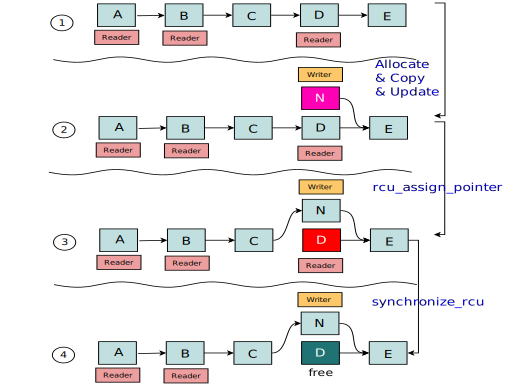
\includegraphics[width=1\textwidth]{fig/rcu/rcu_principle}
    \caption{RCU 예제}
  \label{fig:rcuprinciple}
\end{figure}

%$$$$$$$$$$$$$$$$$$$$$$$$$$$$$$$$$$$$$$$$$$$$$$$$$$$$$$$$$$$$$$$$$$$$$$$$$$$$$$$$
%Paragraph : RCU의 기본 철학
%$$$$$$$$$$$$$$$$$$$$$$$$$$$$$$$$$$$$$$$$$$$$$$$$$$$$$$$$$$$$$$$$$$$$$$$$$$$$$$$$
RCU의 기본 철학은 특정 시점에서 오브젝트를 복제해서 처리한다. 그림~\ref{fig:rcuprinciple}은 
이러한 RCU의 예를 보여준다.
그림에서 1단계에는 A, B, C, D, E 오브젝트 중 A, B, D 오브젝트를 리더들이 읽는 과정을 보여준다.
만약 이 순간 D 오브젝트를 수정하려 하면, RCU는 복사본을 할당 받고, 새로운 값인 오브젝트 N으로 수정을 한다.
그리고 다음 단계에서는 atomic한 연산을 통해서 오브젝트 C와 N을 연결한다. 
이 순간 오브젝트 D를 읽고 이는 리더와 다른 리더들은 아무런 블락 없이 계속 읽기를 수행할 수 있으며,
 동시에 업데이트까지 수행할 수 있어서 성능이 향상된다.
마지막으로 \code{synchroinze\_rcu()} 함수를 통해 리더가 읽기를 마칠 때 까지 기다리고, 읽기가 끝나면 
바로 \code{free()}를 수행한다. 
이 때 마지막 리더가 읽을 때 까지 기다리는 시간을 RCU에서는 grace period라 부른다. 

%$$$$$$$$$$$$$$$$$$$$$$$$$$$$$$$$$$$$$$$$$$$$$$$$$$$$$$$$$$$$$$$$$$$$$$$$$$$$$$$$
%Paragraph : RCU는 기본적으로 3가지 특징
%$$$$$$$$$$$$$$$$$$$$$$$$$$$$$$$$$$$$$$$$$$$$$$$$$$$$$$$$$$$$$$$$$$$$$$$$$$$$$$$$
RCU는 기본적으로 3가지 특징을 가진다. 첫 번째로 Lock-free 리더이다.
실제로 RCU의 리더들은 아무런 락 또는 배리어(barrier)를 소유하지 않고 수행되며, 리드 구간에서는
 per-core 자료구조에 단순히 enter/exit를 기록하여 수행한다. 
따라서, 락 발생하는 캐시 일관성 트래픽이 발생하지 않는다.
두번 째로, Single pointer update이다.
RCU의 writer는 atomic 명령으로 one pointer 업데이트를 수행한다.
이러한 특징으로 인해 여러 리더들과 한가지 업데이터가 동시에 동작할 수 있다.  
마지막으로, RCU는 delayed free를 수행한다.
노드를 바로 free를 하지 않고, 모든 리더들이 리드 구역을 벋어난 경우 까지 
기다린 후 해당 노드를 free한다.
이를 통해 안전하게 노드를 자원 해재할 수 있다. 

\begin{figure}[h]
    \centering
    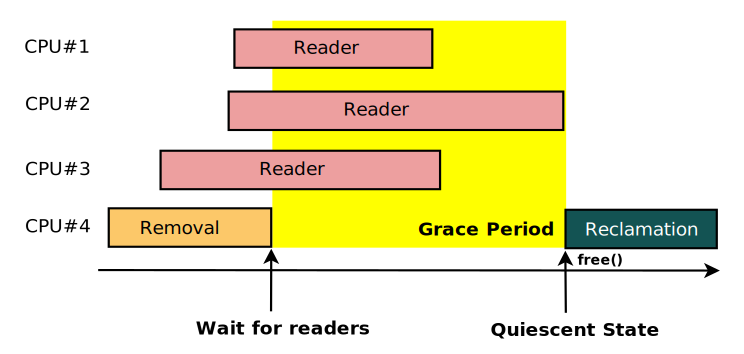
\includegraphics[width=1\textwidth]{fig/rcu/rcu_grace}
    \caption{RCU의 delayed free의 시점}
  \label{fig:rcu_grace}
\end{figure}

그림~\ref{fig:rcu_grace}는 RCU의 delayed free의 시점을 보여준다 . 


%$$$$$$$$$$$$$$$$$$$$$$$$$$$$$$$$$$$$$$$$$$$$$$$$$$$$$$$$$$$$$$$$$$$$$$$$$$$$$$$$
%Paragraph 2: RCU의 grace periad
%$$$$$$$$$$$$$$$$$$$$$$$$$$$$$$$$$$$$$$$$$$$$$$$$$$$$$$$$$$$$$$$$$$$$$$$$$$$$$$$$
RCU는 기본적으로 3가지 특징을 가진다. 첫 번째로 Lock-free 리더이다.
실제로 RCU의 리더들은 아무런 락 또는 배리어(barrier)를 소유하지 않고 수행되며, 리드 구간에서는
 per-core 자료구조에 단순히 enter/exit를 기록하여 수행한다. 
따라서, 락 발생하는 캐시 일관성 트래픽이 발생하지 않는다.
두번 째로, Single pointer update이다.
RCU의 writer는 atomic 명령으로 one pointer 업데이트를 수행한다.
이러한 특징으로 인해 여러 리더들과 한가지 업데이터가 동시에 동작할 수 있다.  
마지막으로, RCU는 delayed free를 수행한다.
노드를 바로 free를 하지 않고, 모든 리더들이 리드 구역을 벋어난 경우 까지 
기다린 후 해당 노드를 free한다.
이를 통해 안전하게 노드를 자원 해재할 수 있다. 

\begin{figure*}[h]
\begin{center}
\inputminted[linenos,fontsize=\footnotesize,
tabsize=4]{c}{src/rcu_list_data.c}
\end{center}
\caption{LDU의 동시적 삽제에 대한 알고리즘.}
\label{fig:gldulogicalupdate}
\end{figure*}



\begin{figure}[h!]
\begin{center}
\inputminted[linenos,fontsize=\footnotesize,
tabsize=4]{c}{src/rcu_list_search.c}
\end{center}
\caption{LDU의 동시적 삽제에 대한 알고리즘.}
\label{fig:gldulogicalupdate}
\end{figure}


\begin{figure}[h!]
\begin{center}
\inputminted[linenos,fontsize=\footnotesize,
tabsize=4]{c}{src/rcu_list_delete.c}
\end{center}
\caption{LDU의 동시적 삽제에 대한 알고리즘.}
\label{fig:gldulogicalupdate}
\end{figure}


%$$$$$$$$$$$$$$$$$$$$$$$$$$$$$$$$$$$$$$$$$$$$$$$$$$$$$$$$$$$$$$$$$$$$$$$$$$$$$$$$
%Paragraph 2: RCU의 예제 source 코드
%$$$$$$$$$$$$$$$$$$$$$$$$$$$$$$$$$$$$$$$$$$$$$$$$$$$$$$$$$$$$$$$$$$$$$$$$$$$$$$$$
RCU는 기본적으로 3가지 특징을 가진다. 첫 번째로 Lock-free 리더이다.
실제로 RCU의 리더들은 아무런 락 또는 배리어(barrier)를 소유하지 않고 수행되며, 리드 구간에서는
 per-core 자료구조에 단순히 enter/exit를 기록하여 수행한다. 
따라서, 락 발생하는 캐시 일관성 트래픽이 발생하지 않는다.
두번 째로, Single pointer update이다.
RCU의 writer는 atomic 명령으로 one pointer 업데이트를 수행한다.
이러한 특징으로 인해 여러 리더들과 한가지 업데이터가 동시에 동작할 수 있다.  
마지막으로, RCU는 delayed free를 수행한다.
노드를 바로 free를 하지 않고, 모든 리더들이 리드 구역을 벋어난 경우 까지 
기다린 후 해당 노드를 free한다.
이를 통해 안전하게 노드를 자원 해재할 수 있다. 



\subsubsection{RLU}

%$$$$$$$$$$$$$$$$$$$$$$$$$$$$$$$$$$$$$$$$$$$$$$$$$$$$$$$$$$$$$$$$$$$$$$$$$$$$$$$$
%Paragraph : RLU가 해결하고자 하는 문제
%$$$$$$$$$$$$$$$$$$$$$$$$$$$$$$$$$$$$$$$$$$$$$$$$$$$$$$$$$$$$$$$$$$$$$$$$$$$$$$$$
RLU는 \ldots
RCU는 기본적으로 3가지 특징을 가진다. 첫 번째로 Lock-free 리더이다.
실제로 RCU의 리더들은 아무런 락 또는 배리어(barrier)를 소유하지 않고 수행되며, 리드 구간에서는
 per-core 자료구조에 단순히 enter/exit를 기록하여 수행한다. 
따라서, 락 발생하는 캐시 일관성 트래픽이 발생하지 않는다.
두번 째로, Single pointer update이다.
RCU의 writer는 atomic 명령으로 one pointer 업데이트를 수행한다.
이러한 특징으로 인해 여러 리더들과 한가지 업데이터가 동시에 동작할 수 있다.  
마지막으로, RCU는 delayed free를 수행한다.
노드를 바로 free를 하지 않고, 모든 리더들이 리드 구역을 벋어난 경우 까지 
기다린 후 해당 노드를 free한다.
이를 통해 안전하게 노드를 자원 해재할 수 있다. 


%$$$$$$$$$$$$$$$$$$$$$$$$$$$$$$$$$$$$$$$$$$$$$$$$$$$$$$$$$$$$$$$$$$$$$$$$$$$$$$$$
%Paragraph : RLU가 해결한 방법
%$$$$$$$$$$$$$$$$$$$$$$$$$$$$$$$$$$$$$$$$$$$$$$$$$$$$$$$$$$$$$$$$$$$$$$$$$$$$$$$$
RCU는 기본적으로 3가지 특징을 가진다. 첫 번째로 Lock-free 리더이다.
실제로 RCU의 리더들은 아무런 락 또는 배리어(barrier)를 소유하지 않고 수행되며, 리드 구간에서는
 per-core 자료구조에 단순히 enter/exit를 기록하여 수행한다. 
따라서, 락 발생하는 캐시 일관성 트래픽이 발생하지 않는다.
두번 째로, Single pointer update이다.
RCU의 writer는 atomic 명령으로 one pointer 업데이트를 수행한다.
이러한 특징으로 인해 여러 리더들과 한가지 업데이터가 동시에 동작할 수 있다.  
마지막으로, RCU는 delayed free를 수행한다.
노드를 바로 free를 하지 않고, 모든 리더들이 리드 구역을 벋어난 경우 까지 
기다린 후 해당 노드를 free한다.
이를 통해 안전하게 노드를 자원 해재할 수 있다. 


\subsubsection{Non-locking synchronization}



%$$$$$$$$$$$$$$$$$$$$$$$$$$$$$$$$$$$$$$$$$$$$$$$$$$$$$$$$$$$$$$$$$$$$$$$$$$$$$$$$
%Paragraph : Non-locking synchronization의 장점
%$$$$$$$$$$$$$$$$$$$$$$$$$$$$$$$$$$$$$$$$$$$$$$$$$$$$$$$$$$$$$$$$$$$$$$$$$$$$$$$$
Non-blocking synchronization은 장점은 여러 스레드들이 락 기반으로 자원을 관리함에 따라
 발생하는 문제를 해결할 수 있다. 
가장 큰 장점은 스레드 또는 프로세스가 락 때문에 기다리는 시간을 제거할 수 있다.
이 것은 락을 얻기 위해 기다리는 시간을 최소화 할 뿐만 아니라 무한 루프 때문에 무한정 기다리는 
데드락 같은 상황까지 제거 할 수 있다. 
다음으로 모든 락은 락 자체의 오버헤드를 가지고 있는데 이것을 제거할 수 있다. 
예를 들어 코어 수가 증가 할 수록 락 자체를 얻기 위해 원자적 명령을 이용한느데 이것은 캐시 일관성 트래픽을 
발생한다. 
이와 같이 Non-blocking 방법은 이러한 락 자체가 가지고 있는 문제점인 데드락(deadlock), 라이브락(livelock), 
우선순위 역전현상(priority inversion)등을 제거 할 수 있다. 

이러한 Non-blocking synchronization 기법을 사용하는 lock-free 자료 구조들은 성능을 향상 시킬 수 있다. 
그 이유는 멀티코어 환경에서 공유되는 데이터를 접근하기 위해 직렬화 되는 부분이 매우 짧기 때문이다. 

\begin{figure}[h!]
    \centering
    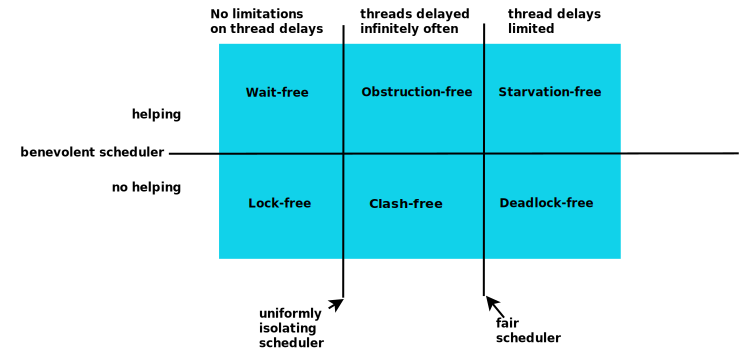
\includegraphics[width=1\textwidth]{fig/NBS/NBS}
    \caption{Non-locking synchronization}
  \label{fig:NBS}
\end{figure}


%$$$$$$$$$$$$$$$$$$$$$$$$$$$$$$$$$$$$$$$$$$$$$$$$$$$$$$$$$$$$$$$$$$$$$$$$$$$$$$$$
%Paragraph : Non-locking synchronization 알고리즘 종류 1 
%$$$$$$$$$$$$$$$$$$$$$$$$$$$$$$$$$$$$$$$$$$$$$$$$$$$$$$$$$$$$$$$$$$$$$$$$$$$$$$$$
Non-blocking synchronization은 장점은 여러 스레드들이 락 기반으로 자원을 관리함에 따라
 발생하는 문제를 해결할 수 있다. 
가장 큰 장점은 스레드 또는 프로세스가 락 때문에 기다리는 시간을 제거할 수 있다.
이 것은 락을 얻기 위해 기다리는 시간을 최소화 할 뿐만 아니라 무한 루프 때문에 무한정 기다리는 
데드락 같은 상황까지 제거 할 수 있다. 
다음으로 모든 락은 락 자체의 오버헤드를 가지고 있는데 이것을 제거할 수 있다. 
예를 들어 코어 수가 증가 할 수록 락 자체를 얻기 위해 원자적 명령을 이용한느데 이것은 캐시 일관성 트래픽을 
발생한다. 
이와 같이 Non-blocking 방법은 이러한 락 자체가 가지고 있는 문제점인 데드락(deadlock), 라이브락(livelock), 
우선순위 역전현상(priority inversion)등을 제거 할 수 있다. 
이러한 Non-blocking synchronization 기법을 사용하는 lock-free 자료 구조들은 성능을 향상 시킬 수 있다. 
그 이유는 멀티코어 환경에서 공유되는 데이터를 접근하기 위해 직렬화 되는 부분이 매우 짧기 때문이다. 


%$$$$$$$$$$$$$$$$$$$$$$$$$$$$$$$$$$$$$$$$$$$$$$$$$$$$$$$$$$$$$$$$$$$$$$$$$$$$$$$$
%Paragraph :  Non-locking synchronization 알고리즘 종류 2
%$$$$$$$$$$$$$$$$$$$$$$$$$$$$$$$$$$$$$$$$$$$$$$$$$$$$$$$$$$$$$$$$$$$$$$$$$$$$$$$$
Non-blocking synchronization은 장점은 여러 스레드들이 락 기반으로 자원을 관리함에 따라
 발생하는 문제를 해결할 수 있다. 
가장 큰 장점은 스레드 또는 프로세스가 락 때문에 기다리는 시간을 제거할 수 있다.
이 것은 락을 얻기 위해 기다리는 시간을 최소화 할 뿐만 아니라 무한 루프 때문에 무한정 기다리는 
데드락 같은 상황까지 제거 할 수 있다. 
다음으로 모든 락은 락 자체의 오버헤드를 가지고 있는데 이것을 제거할 수 있다. 
예를 들어 코어 수가 증가 할 수록 락 자체를 얻기 위해 원자적 명령을 이용한느데 이것은 캐시 일관성 트래픽을 
발생한다. 
이와 같이 Non-blocking 방법은 이러한 락 자체가 가지고 있는 문제점인 데드락(deadlock), 라이브락(livelock), 
우선순위 역전현상(priority inversion)등을 제거 할 수 있다. 
이러한 Non-blocking synchronization 기법을 사용하는 lock-free 자료 구조들은 성능을 향상 시킬 수 있다. 
그 이유는 멀티코어 환경에서 공유되는 데이터를 접근하기 위해 직렬화 되는 부분이 매우 짧기 때문이다. 


이러한 장점을 가진 Non-blockig Algortithm은 그림 \ref{fig:nonblockingstack}과 같이 구현되어 있다. 


\begin{figure}[h!]
\begin{center}
\inputminted[linenos,fontsize=\footnotesize,
tabsize=4]{c}{src/lockfree_stack.c}
\end{center}
\caption{간단한 Non-blocking 스택 알고리즘.}
\label{fig:nonblockingstack}
\end{figure}


%$$$$$$$$$$$$$$$$$$$$$$$$$$$$$$$$$$$$$$$$$$$$$$$$$$$$$$$$$$$$$$$$$$$$$$$$$$$$$$$$
%Paragraph : 심플 스택 알고리즘 설명
%$$$$$$$$$$$$$$$$$$$$$$$$$$$$$$$$$$$$$$$$$$$$$$$$$$$$$$$$$$$$$$$$$$$$$$$$$$$$$$$$
Non-blocking synchronization은 장점은 여러 스레드들이 락 기반으로 자원을 관리함에 따라
 발생하는 문제를 해결할 수 있다. 
가장 큰 장점은 스레드 또는 프로세스가 락 때문에 기다리는 시간을 제거할 수 있다.
이 것은 락을 얻기 위해 기다리는 시간을 최소화 할 뿐만 아니라 무한 루프 때문에 무한정 기다리는 
데드락 같은 상황까지 제거 할 수 있다. 
다음으로 모든 락은 락 자체의 오버헤드를 가지고 있는데 이것을 제거할 수 있다. 
예를 들어 코어 수가 증가 할 수록 락 자체를 얻기 위해 원자적 명령을 이용한느데 이것은 캐시 일관성 트래픽을 
발생한다. 
이와 같이 Non-blocking 방법은 이러한 락 자체가 가지고 있는 문제점인 데드락(deadlock), 라이브락(livelock), 
우선순위 역전현상(priority inversion)등을 제거 할 수 있다. 
이러한 Non-blocking synchronization 기법을 사용하는 lock-free 자료 구조들은 성능을 향상 시킬 수 있다. 
그 이유는 멀티코어 환경에서 공유되는 데이터를 접근하기 위해 직렬화 되는 부분이 매우 짧기 때문이다. 


%Hash tables
  %Used for shared caches (name cache, buffer cache)
   % map block# to block
  %Implementations
    %one lock per hash table (bad scaling)
     % lots of unintended sharing
    %one lock per bucket (better scaling)
     % blocks that map to same buck share unintendedly
    %lock-free lists per bucket (see below)
%      little unintended sharing
%      case: search with on list, while someone is removing
      


%Challenge: Memory reuse (ABA problem)
%stack contains three elements
%top -> A -> B -> C
  %CPU 1 about to pop off the top of the stack,
    %preempted just before cmpxchg(top, A, B)
  %CPU 2 pops off A, B, frees both of them
   % top -> C
  %CPU 2 allocates another item (malloc reuses A) and pushes onto stack
    %top -> A -> C
  %CPU 1: cmpxchg succeeds, stack now looks like
    %top -> B -> C
  %this is called the "ABA problem"  
   %(memory switches from A-state to B-state and back to A-state without being
   % able to tell)


%Solution: delay freeing until safe
   %E.g., Arrange time in epochs
   %Free when all processors have left previous

  

%Challenge: involves true sharing
  %Many resources in kernel are reference counted
  %Often a scaling bottleneck (once unintended sharing is removed)


%$$$$$$$$$$$$$$$$$$$$$$$$$$$$$$$$$$$$$$$$$$$$$$$$$$$$$$$$$$$$$$$$$$$$$$$$$$$$$$$$
%Paragraph : ABA 문제 설명
%$$$$$$$$$$$$$$$$$$$$$$$$$$$$$$$$$$$$$$$$$$$$$$$$$$$$$$$$$$$$$$$$$$$$$$$$$$$$$$$$
Non-blocking synchronization은 장점은 여러 스레드들이 락 기반으로 자원을 관리함에 따라
 발생하는 문제를 해결할 수 있다. 
가장 큰 장점은 스레드 또는 프로세스가 락 때문에 기다리는 시간을 제거할 수 있다.
이 것은 락을 얻기 위해 기다리는 시간을 최소화 할 뿐만 아니라 무한 루프 때문에 무한정 기다리는 
데드락 같은 상황까지 제거 할 수 있다. 
다음으로 모든 락은 락 자체의 오버헤드를 가지고 있는데 이것을 제거할 수 있다. 
예를 들어 코어 수가 증가 할 수록 락 자체를 얻기 위해 원자적 명령을 이용한느데 이것은 캐시 일관성 트래픽을 
발생한다. 
이와 같이 Non-blocking 방법은 이러한 락 자체가 가지고 있는 문제점인 데드락(deadlock), 라이브락(livelock), 
우선순위 역전현상(priority inversion)등을 제거 할 수 있다. 
이러한 Non-blocking synchronization 기법을 사용하는 lock-free 자료 구조들은 성능을 향상 시킬 수 있다. 
그 이유는 멀티코어 환경에서 공유되는 데이터를 접근하기 위해 직렬화 되는 부분이 매우 짧기 때문이다. 



\subsection{확장성 있는 자료구조}

\subsubsection{Harris Linked List}


Non-blocking 알고리즘 중 대표적인 알고리즘 중 하나는 Harris Linked List이다. 
%$$$$$$$$$$$$$$$$$$$$$$$$$$$$$$$$$$$$$$$$$$$$$$$$$$$$$$$$$$$$$$$$$$$$$$$$$$$$$$$$
%Paragraph 2: harris 알고리즘 설명
%$$$$$$$$$$$$$$$$$$$$$$$$$$$$$$$$$$$$$$$$$$$$$$$$$$$$$$$$$$$$$$$$$$$$$$$$$$$$$$$$
Non-blocking synchronization은 장점은 여러 스레드들이 락 기반으로 자원을 관리함에 따라
 발생하는 문제를 해결할 수 있다. 
가장 큰 장점은 스레드 또는 프로세스가 락 때문에 기다리는 시간을 제거할 수 있다.
이 것은 락을 얻기 위해 기다리는 시간을 최소화 할 뿐만 아니라 무한 루프 때문에 무한정 기다리는 
데드락 같은 상황까지 제거 할 수 있다. 
다음으로 모든 락은 락 자체의 오버헤드를 가지고 있는데 이것을 제거할 수 있다. 
예를 들어 코어 수가 증가 할 수록 락 자체를 얻기 위해 원자적 명령을 이용한느데 이것은 캐시 일관성 트래픽을 
발생한다. 
이와 같이 Non-blocking 방법은 이러한 락 자체가 가지고 있는 문제점인 데드락(deadlock), 라이브락(livelock), 
우선순위 역전현상(priority inversion)등을 제거 할 수 있다. 
이러한 Non-blocking synchronization 기법을 사용하는 lock-free 자료 구조들은 성능을 향상 시킬 수 있다. 
그 이유는 멀티코어 환경에서 공유되는 데이터를 접근하기 위해 직렬화 되는 부분이 매우 짧기 때문이다. 



\begin{figure}[h!]
    \centering
    \includegraphics[width=1\textwidth]{fig/harris/harris}
    \caption{Harris 삭제}
  \label{fig:harris}
\end{figure}


%$$$$$$$$$$$$$$$$$$$$$$$$$$$$$$$$$$$$$$$$$$$$$$$$$$$$$$$$$$$$$$$$$$$$$$$$$$$$$$$$
%Paragraph 2: 그림 설명
%$$$$$$$$$$$$$$$$$$$$$$$$$$$$$$$$$$$$$$$$$$$$$$$$$$$$$$$$$$$$$$$$$$$$$$$$$$$$$$$$
Non-blocking synchronization은 장점은 여러 스레드들이 락 기반으로 자원을 관리함에 따라
 발생하는 문제를 해결할 수 있다. 
가장 큰 장점은 스레드 또는 프로세스가 락 때문에 기다리는 시간을 제거할 수 있다.
이 것은 락을 얻기 위해 기다리는 시간을 최소화 할 뿐만 아니라 무한 루프 때문에 무한정 기다리는 
데드락 같은 상황까지 제거 할 수 있다. 
다음으로 모든 락은 락 자체의 오버헤드를 가지고 있는데 이것을 제거할 수 있다. 
예를 들어 코어 수가 증가 할 수록 락 자체를 얻기 위해 원자적 명령을 이용한느데 이것은 캐시 일관성 트래픽을 
발생한다. 
이와 같이 Non-blocking 방법은 이러한 락 자체가 가지고 있는 문제점인 데드락(deadlock), 라이브락(livelock), 
우선순위 역전현상(priority inversion)등을 제거 할 수 있다. 
이러한 Non-blocking synchronization 기법을 사용하는 lock-free 자료 구조들은 성능을 향상 시킬 수 있다. 
그 이유는 멀티코어 환경에서 공유되는 데이터를 접근하기 위해 직렬화 되는 부분이 매우 짧기 때문이다. 




%$$$$$$$$$$$$$$$$$$$$$$$$$$$$$$$$$$$$$$$$$$$$$$$$$$$$$$$$$$$$$$$$$$$$$$$$$$$$$$$$
%Paragraph 2: 코드 설명
%$$$$$$$$$$$$$$$$$$$$$$$$$$$$$$$$$$$$$$$$$$$$$$$$$$$$$$$$$$$$$$$$$$$$$$$$$$$$$$$$
Non-blocking synchronization은 장점은 여러 스레드들이 락 기반으로 자원을 관리함에 따라
 발생하는 문제를 해결할 수 있다. 
가장 큰 장점은 스레드 또는 프로세스가 락 때문에 기다리는 시간을 제거할 수 있다.
이 것은 락을 얻기 위해 기다리는 시간을 최소화 할 뿐만 아니라 무한 루프 때문에 무한정 기다리는 
데드락 같은 상황까지 제거 할 수 있다. 
다음으로 모든 락은 락 자체의 오버헤드를 가지고 있는데 이것을 제거할 수 있다. 
예를 들어 코어 수가 증가 할 수록 락 자체를 얻기 위해 원자적 명령을 이용한느데 이것은 캐시 일관성 트래픽을 
발생한다. 
이와 같이 Non-blocking 방법은 이러한 락 자체가 가지고 있는 문제점인 데드락(deadlock), 라이브락(livelock), 
우선순위 역전현상(priority inversion)등을 제거 할 수 있다. 
이러한 Non-blocking synchronization 기법을 사용하는 lock-free 자료 구조들은 성능을 향상 시킬 수 있다. 
그 이유는 멀티코어 환경에서 공유되는 데이터를 접근하기 위해 직렬화 되는 부분이 매우 짧기 때문이다. 





%\subsubsection{Time-stamp stack}




%\newpage
\section{하드웨어}
\label{sec:hwrelated}

\subsection{캐시 일관성(Cache Coherency)}



병렬화를 위한 캐시는\ldots 




\subsection{원자적 명령(Atomic Operations)}

원자적 명령은\ldots



\subsection{메모리 배리어(Memory Barriers)}

메모리 배리어는\ldots








